\chapter[Comparison of one- and two-b-jet samples in CRTop]{Comparison of one- and two-$b$-jet samples in $\CRTop$}
\label{app:ch8_topcr_1b2b}

The kinematic shapes in the one- and two-$b$-jet $\CRTop$ samples are compared to check their use in a common CR.
The simulated $\mT$ and $m_{b\hadtau}$ distributions are normalised to unit area, so this comparison tests the shapes independently of their event yields.
The electron and muon channels are examined separately in both topologies, as shown in Figures~\ref{fig:ch8_top_1b2b_mt} and~\ref{fig:ch8_top_1b2b_mass}.
No large shape difference is observed.
The inclusive $N_b\geq1$ selection is therefore used to improve the statistical precision of the top-quark background constraint.

\begin{figure}[htpb]
    \centering
    \begin{subfigure}{0.49\linewidth}
        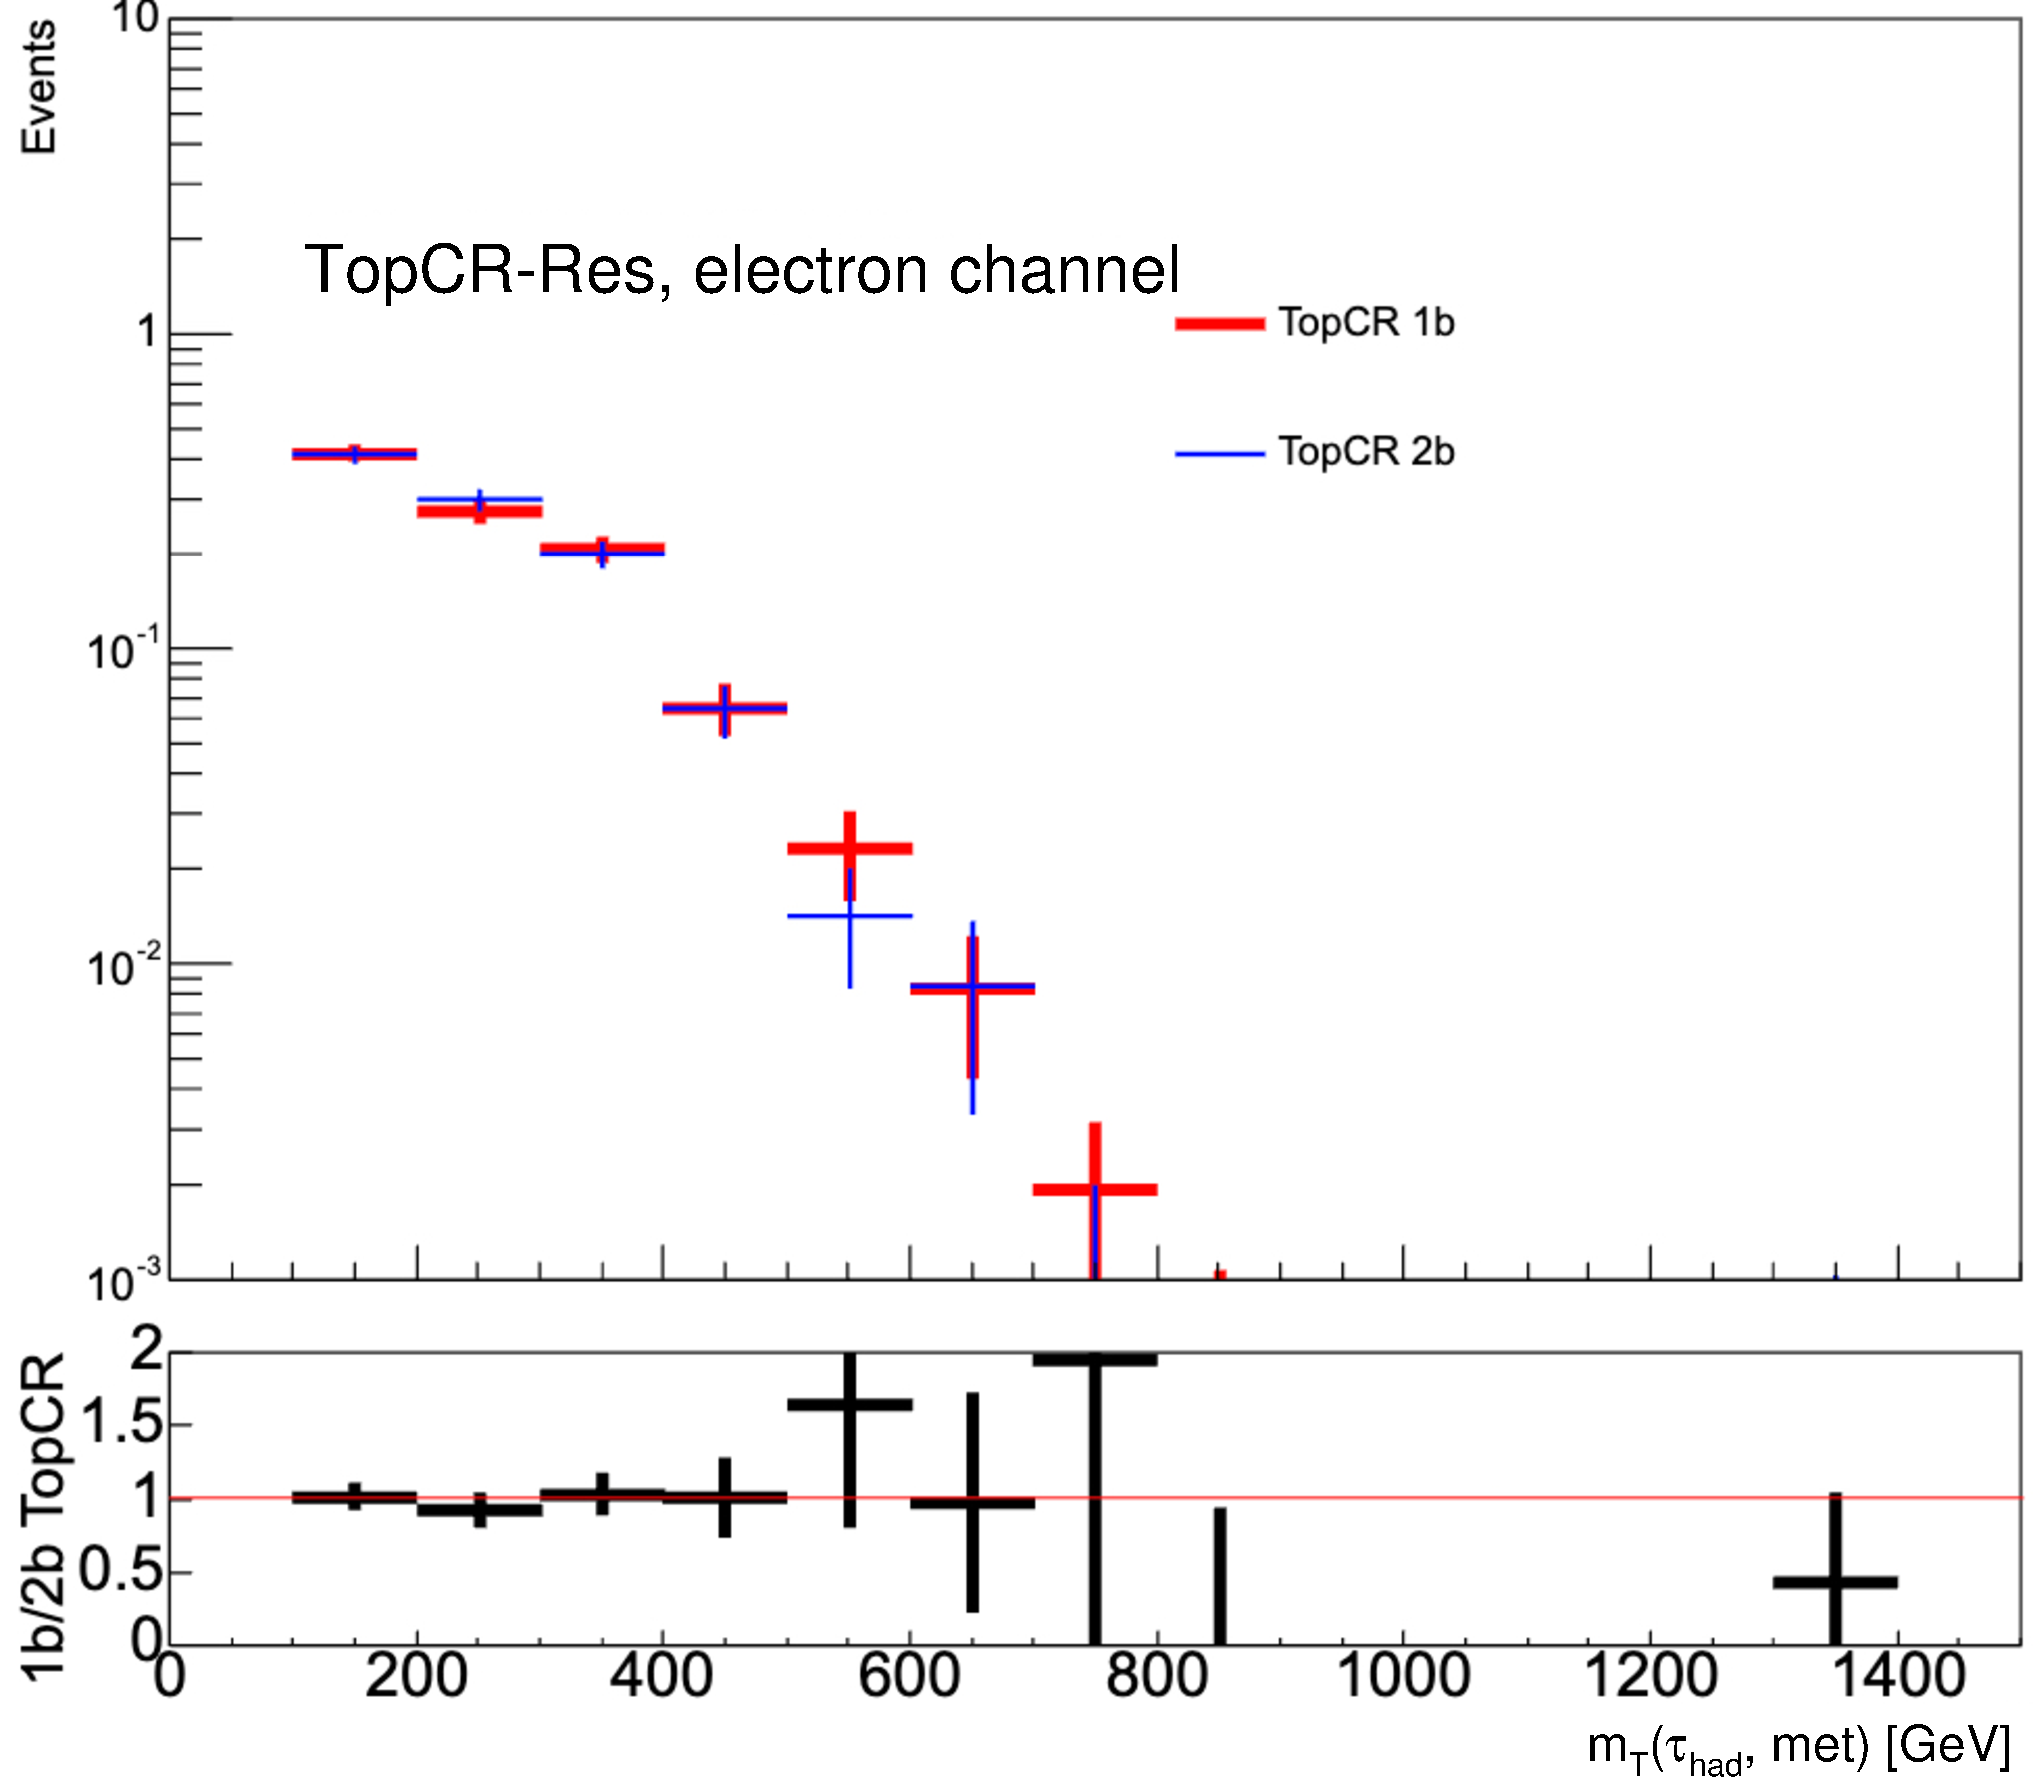
\includegraphics[width=\linewidth]{Figs/CH8/studies/TopCR_1e_sch_mT.pdf}
        \caption[]{$e$ channel, Res.}
    \end{subfigure}\hfill
    \begin{subfigure}{0.49\linewidth}
        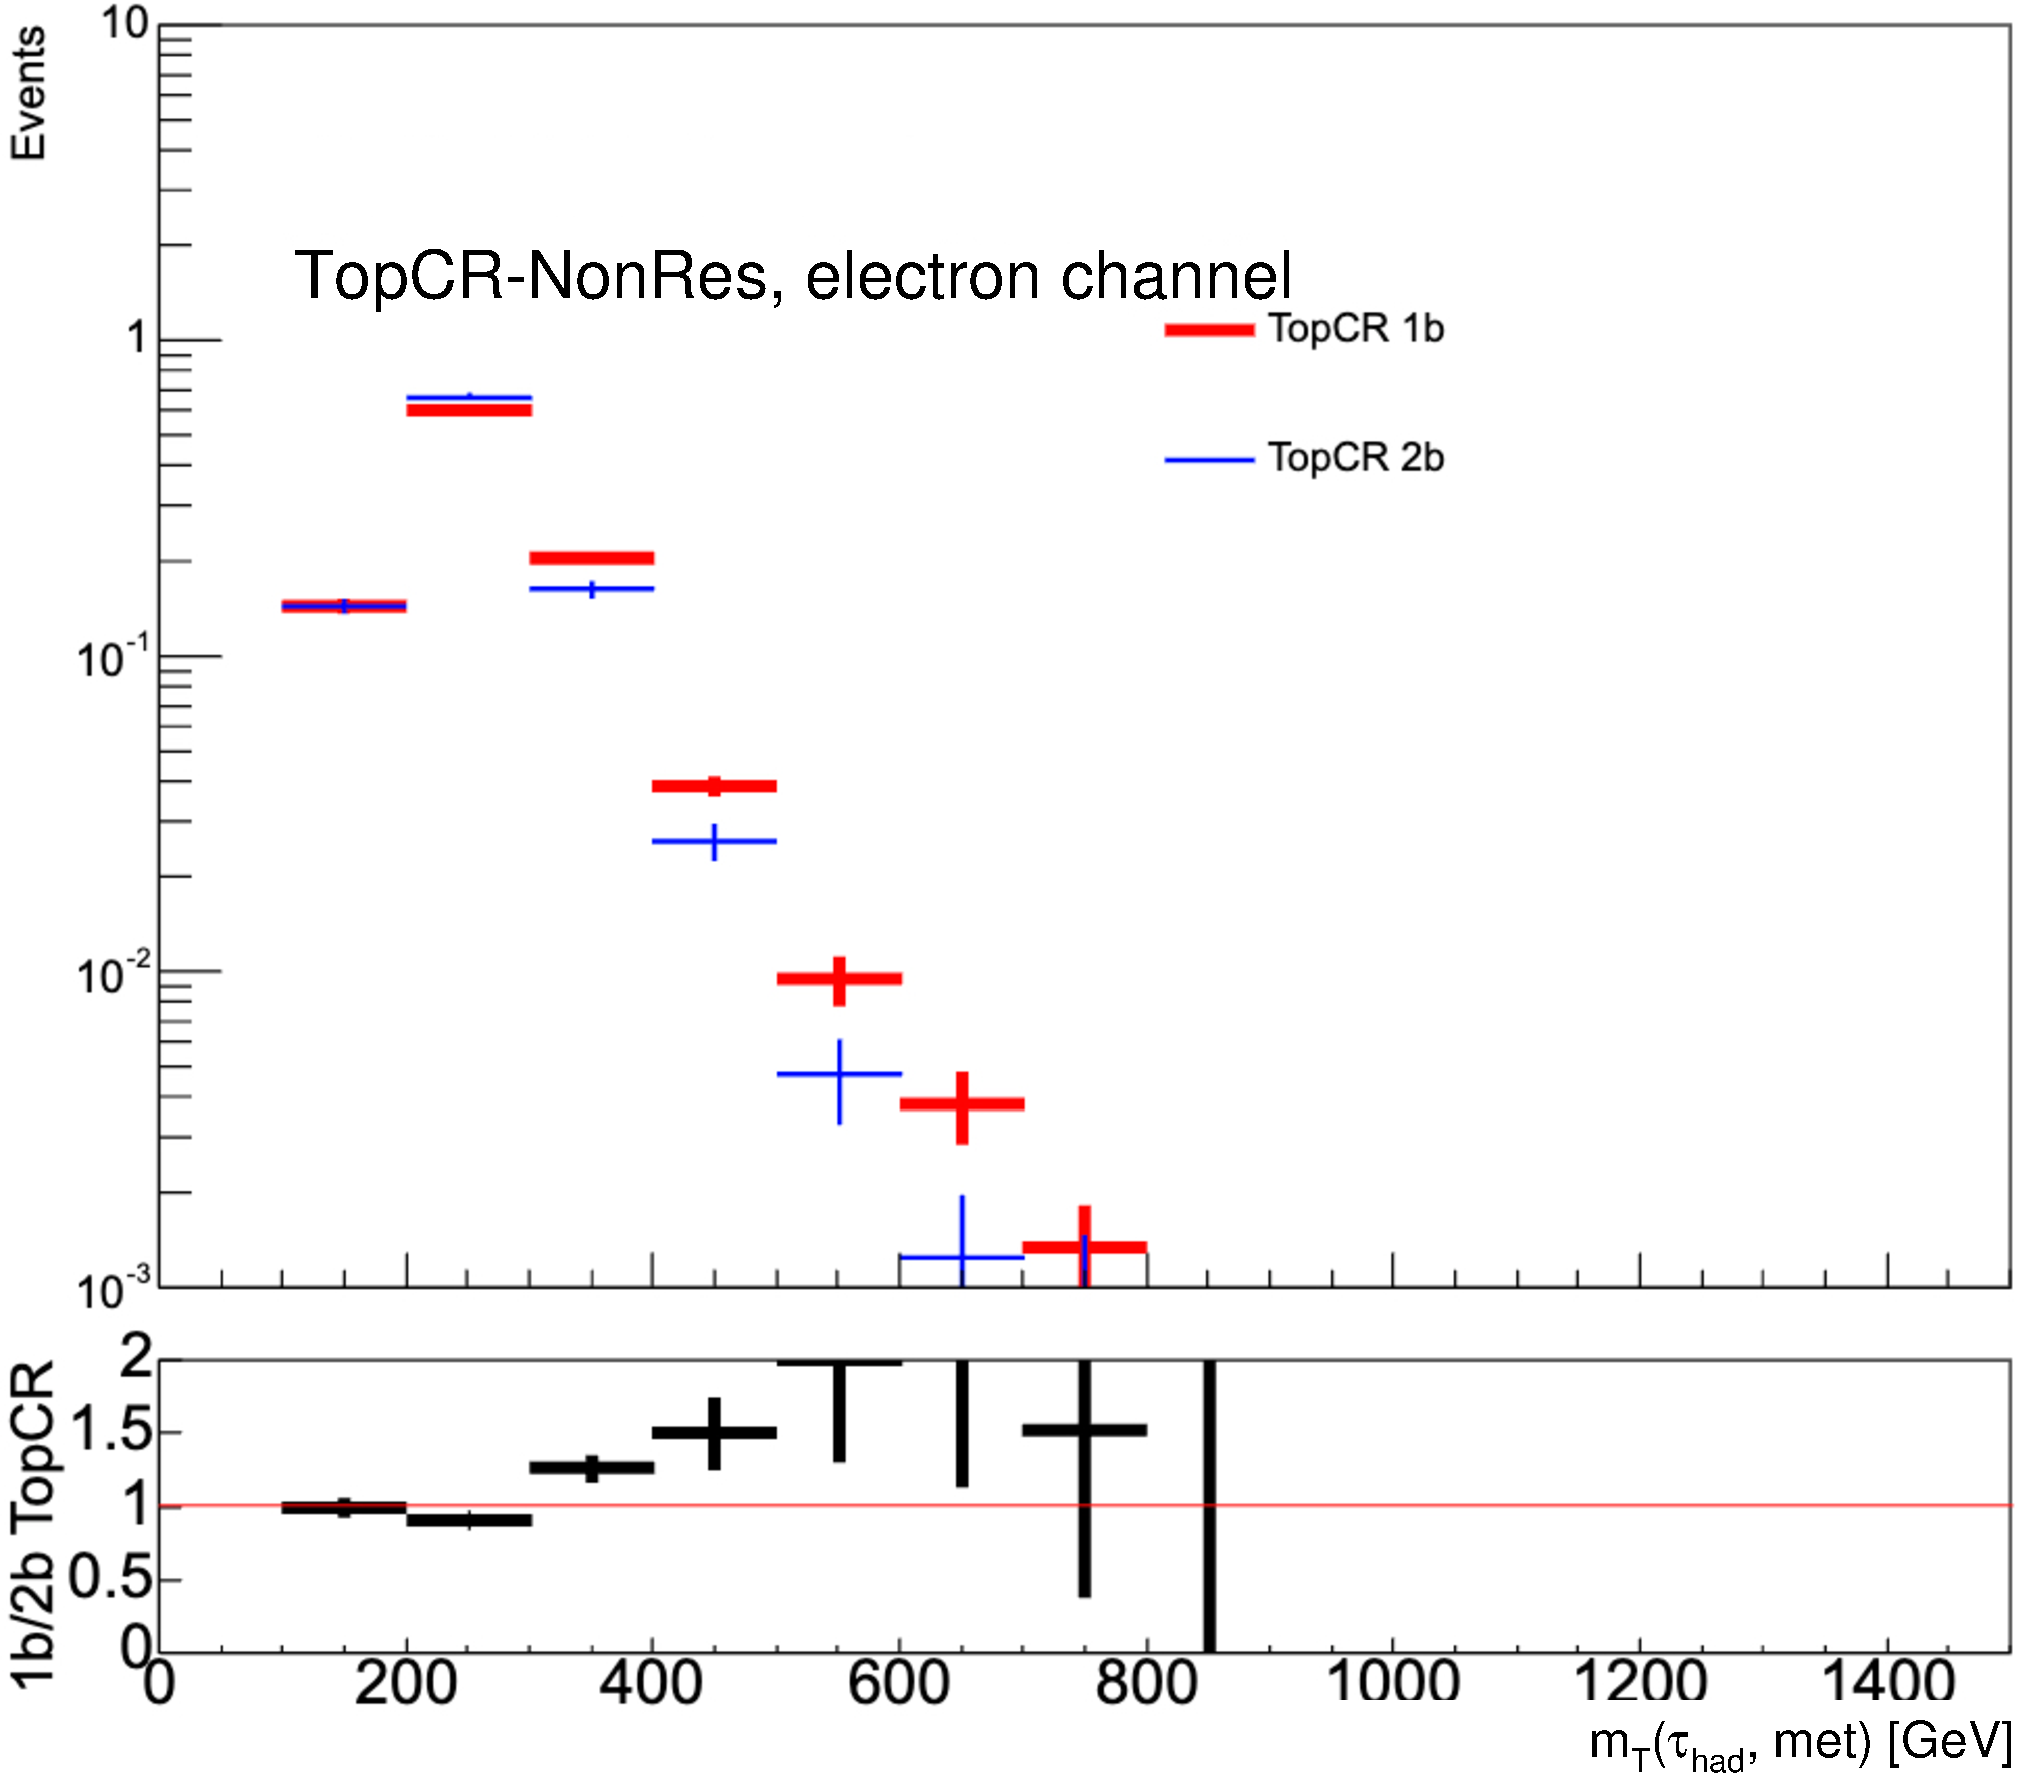
\includegraphics[width=\linewidth]{Figs/CH8/studies/TopCR_1e_tch_mT.pdf}
        \caption[]{$e$ channel, NonRes.}
    \end{subfigure}\\
    \begin{subfigure}{0.49\linewidth}
        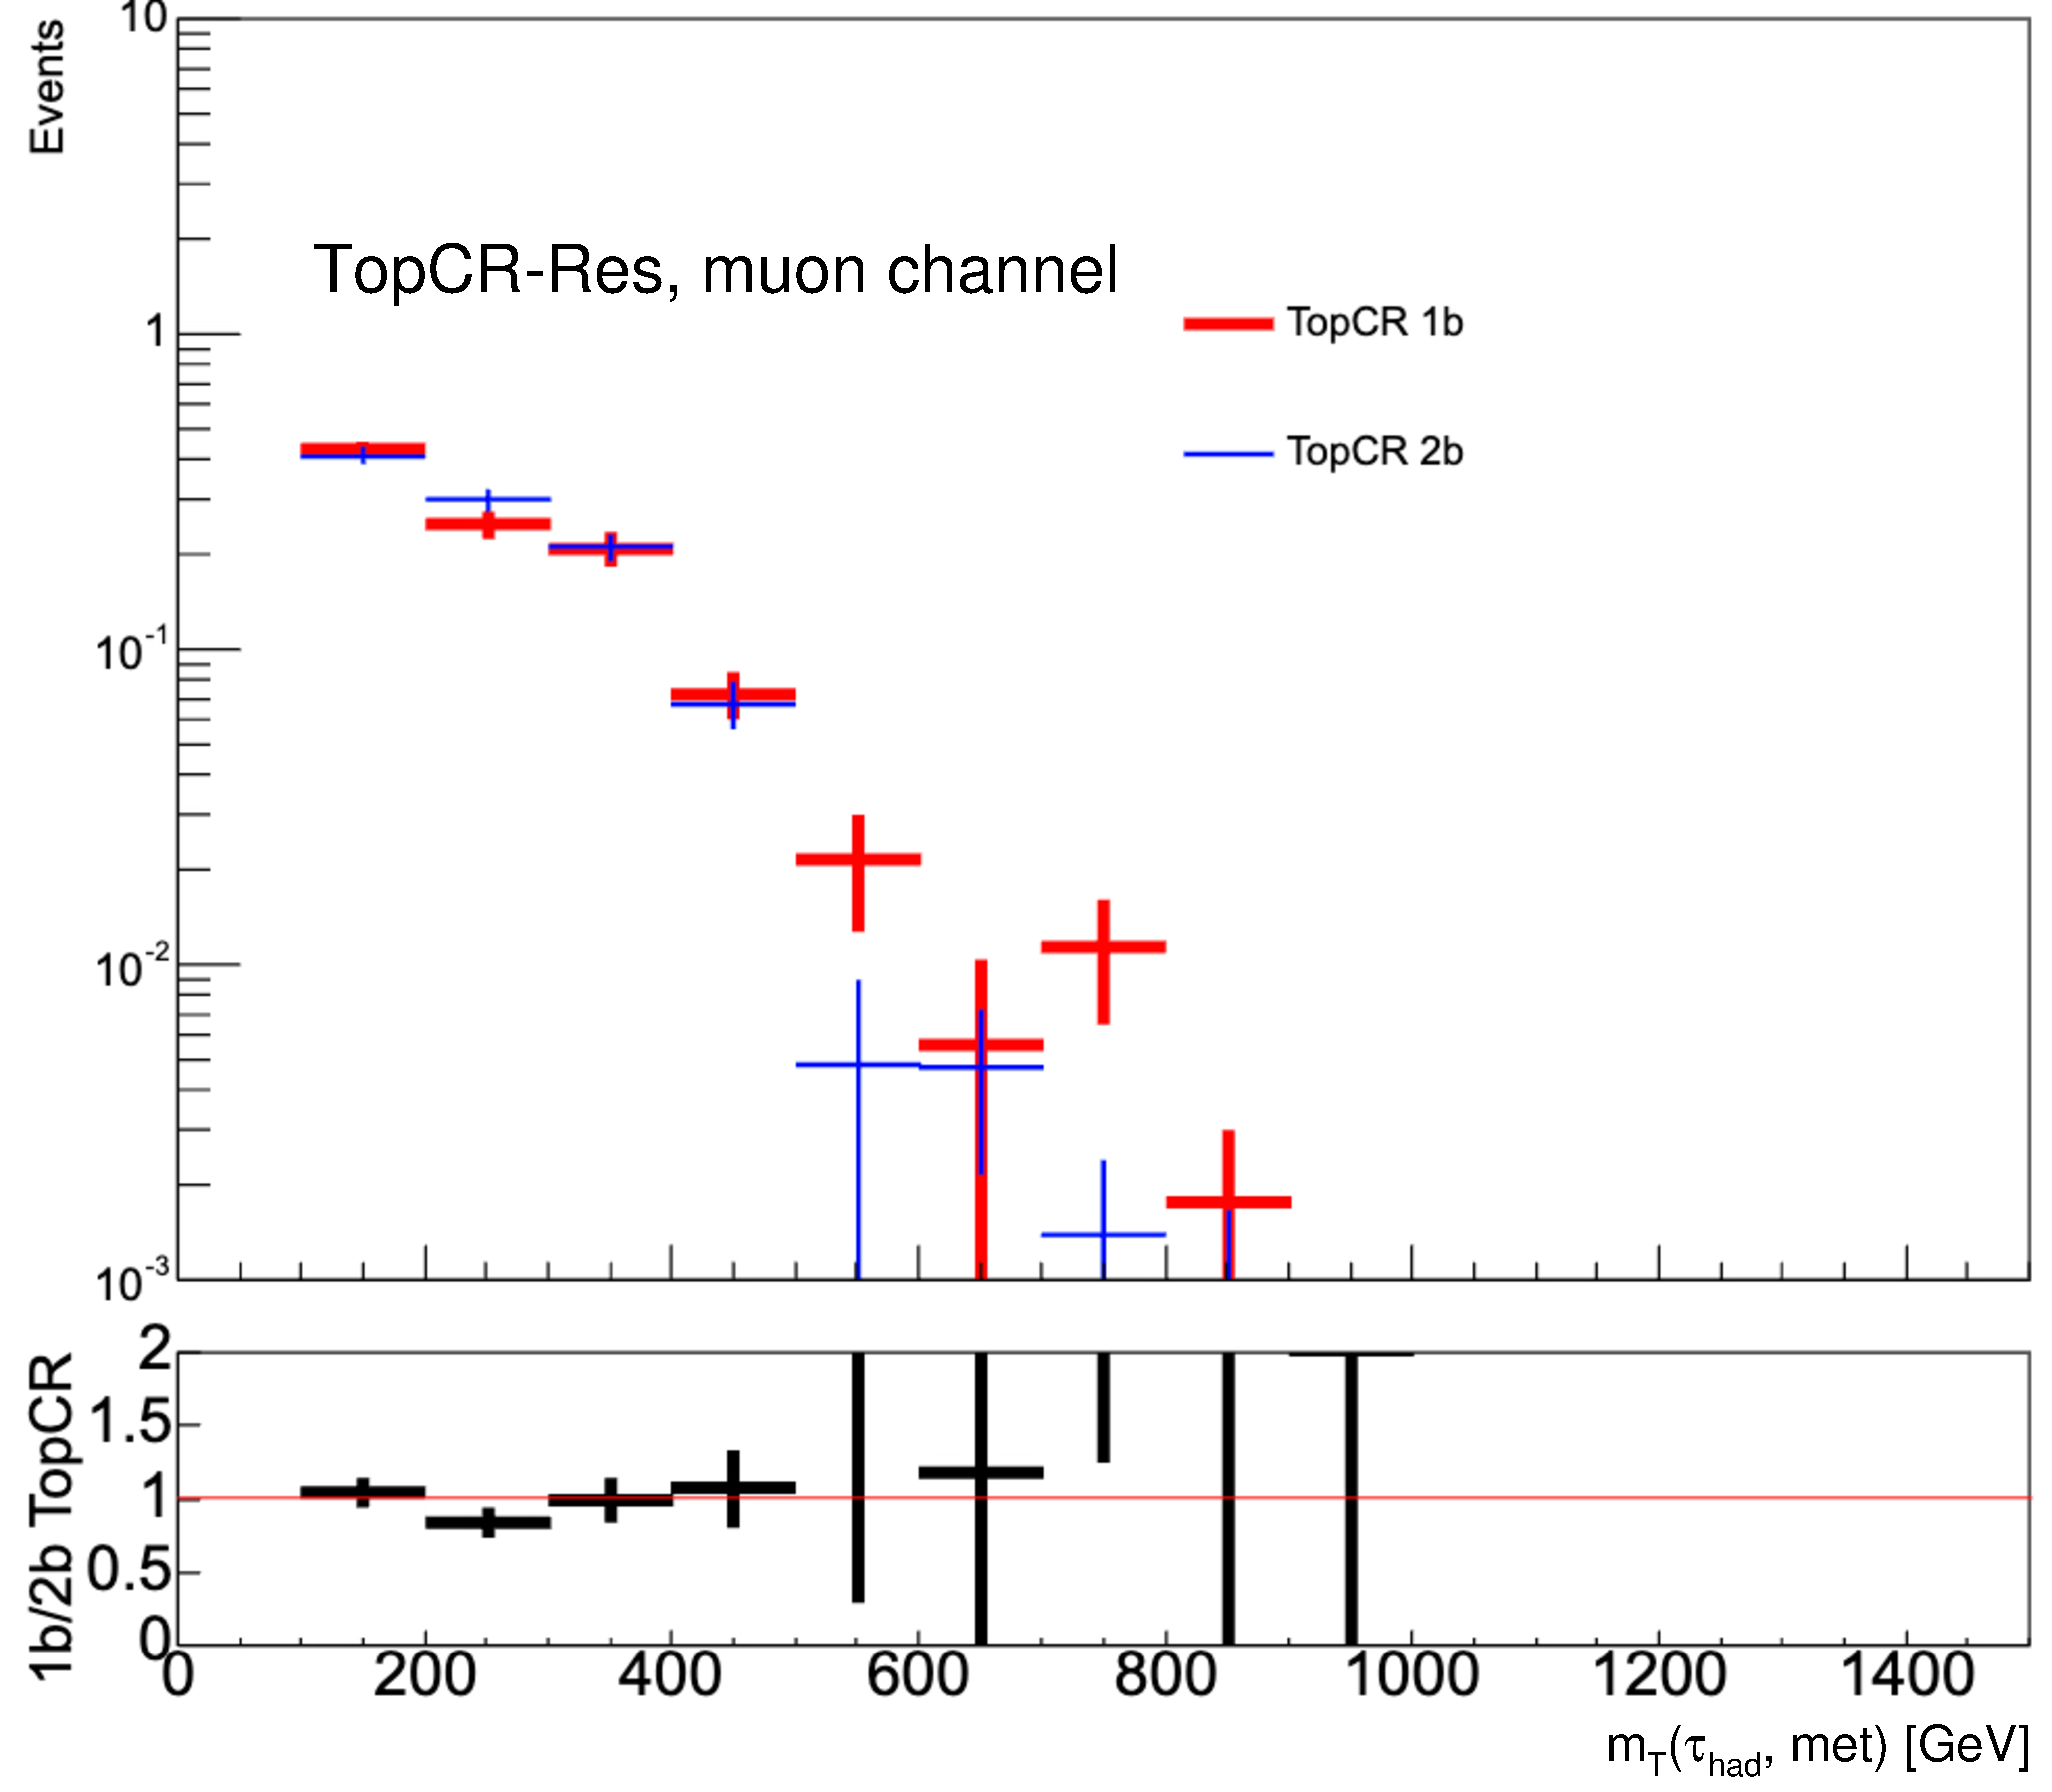
\includegraphics[width=\linewidth]{Figs/CH8/studies/TopCR_1mu_sch_mT.pdf}
        \caption[]{$\mu$ channel, Res.}
    \end{subfigure}\hfill
    \begin{subfigure}{0.49\linewidth}
        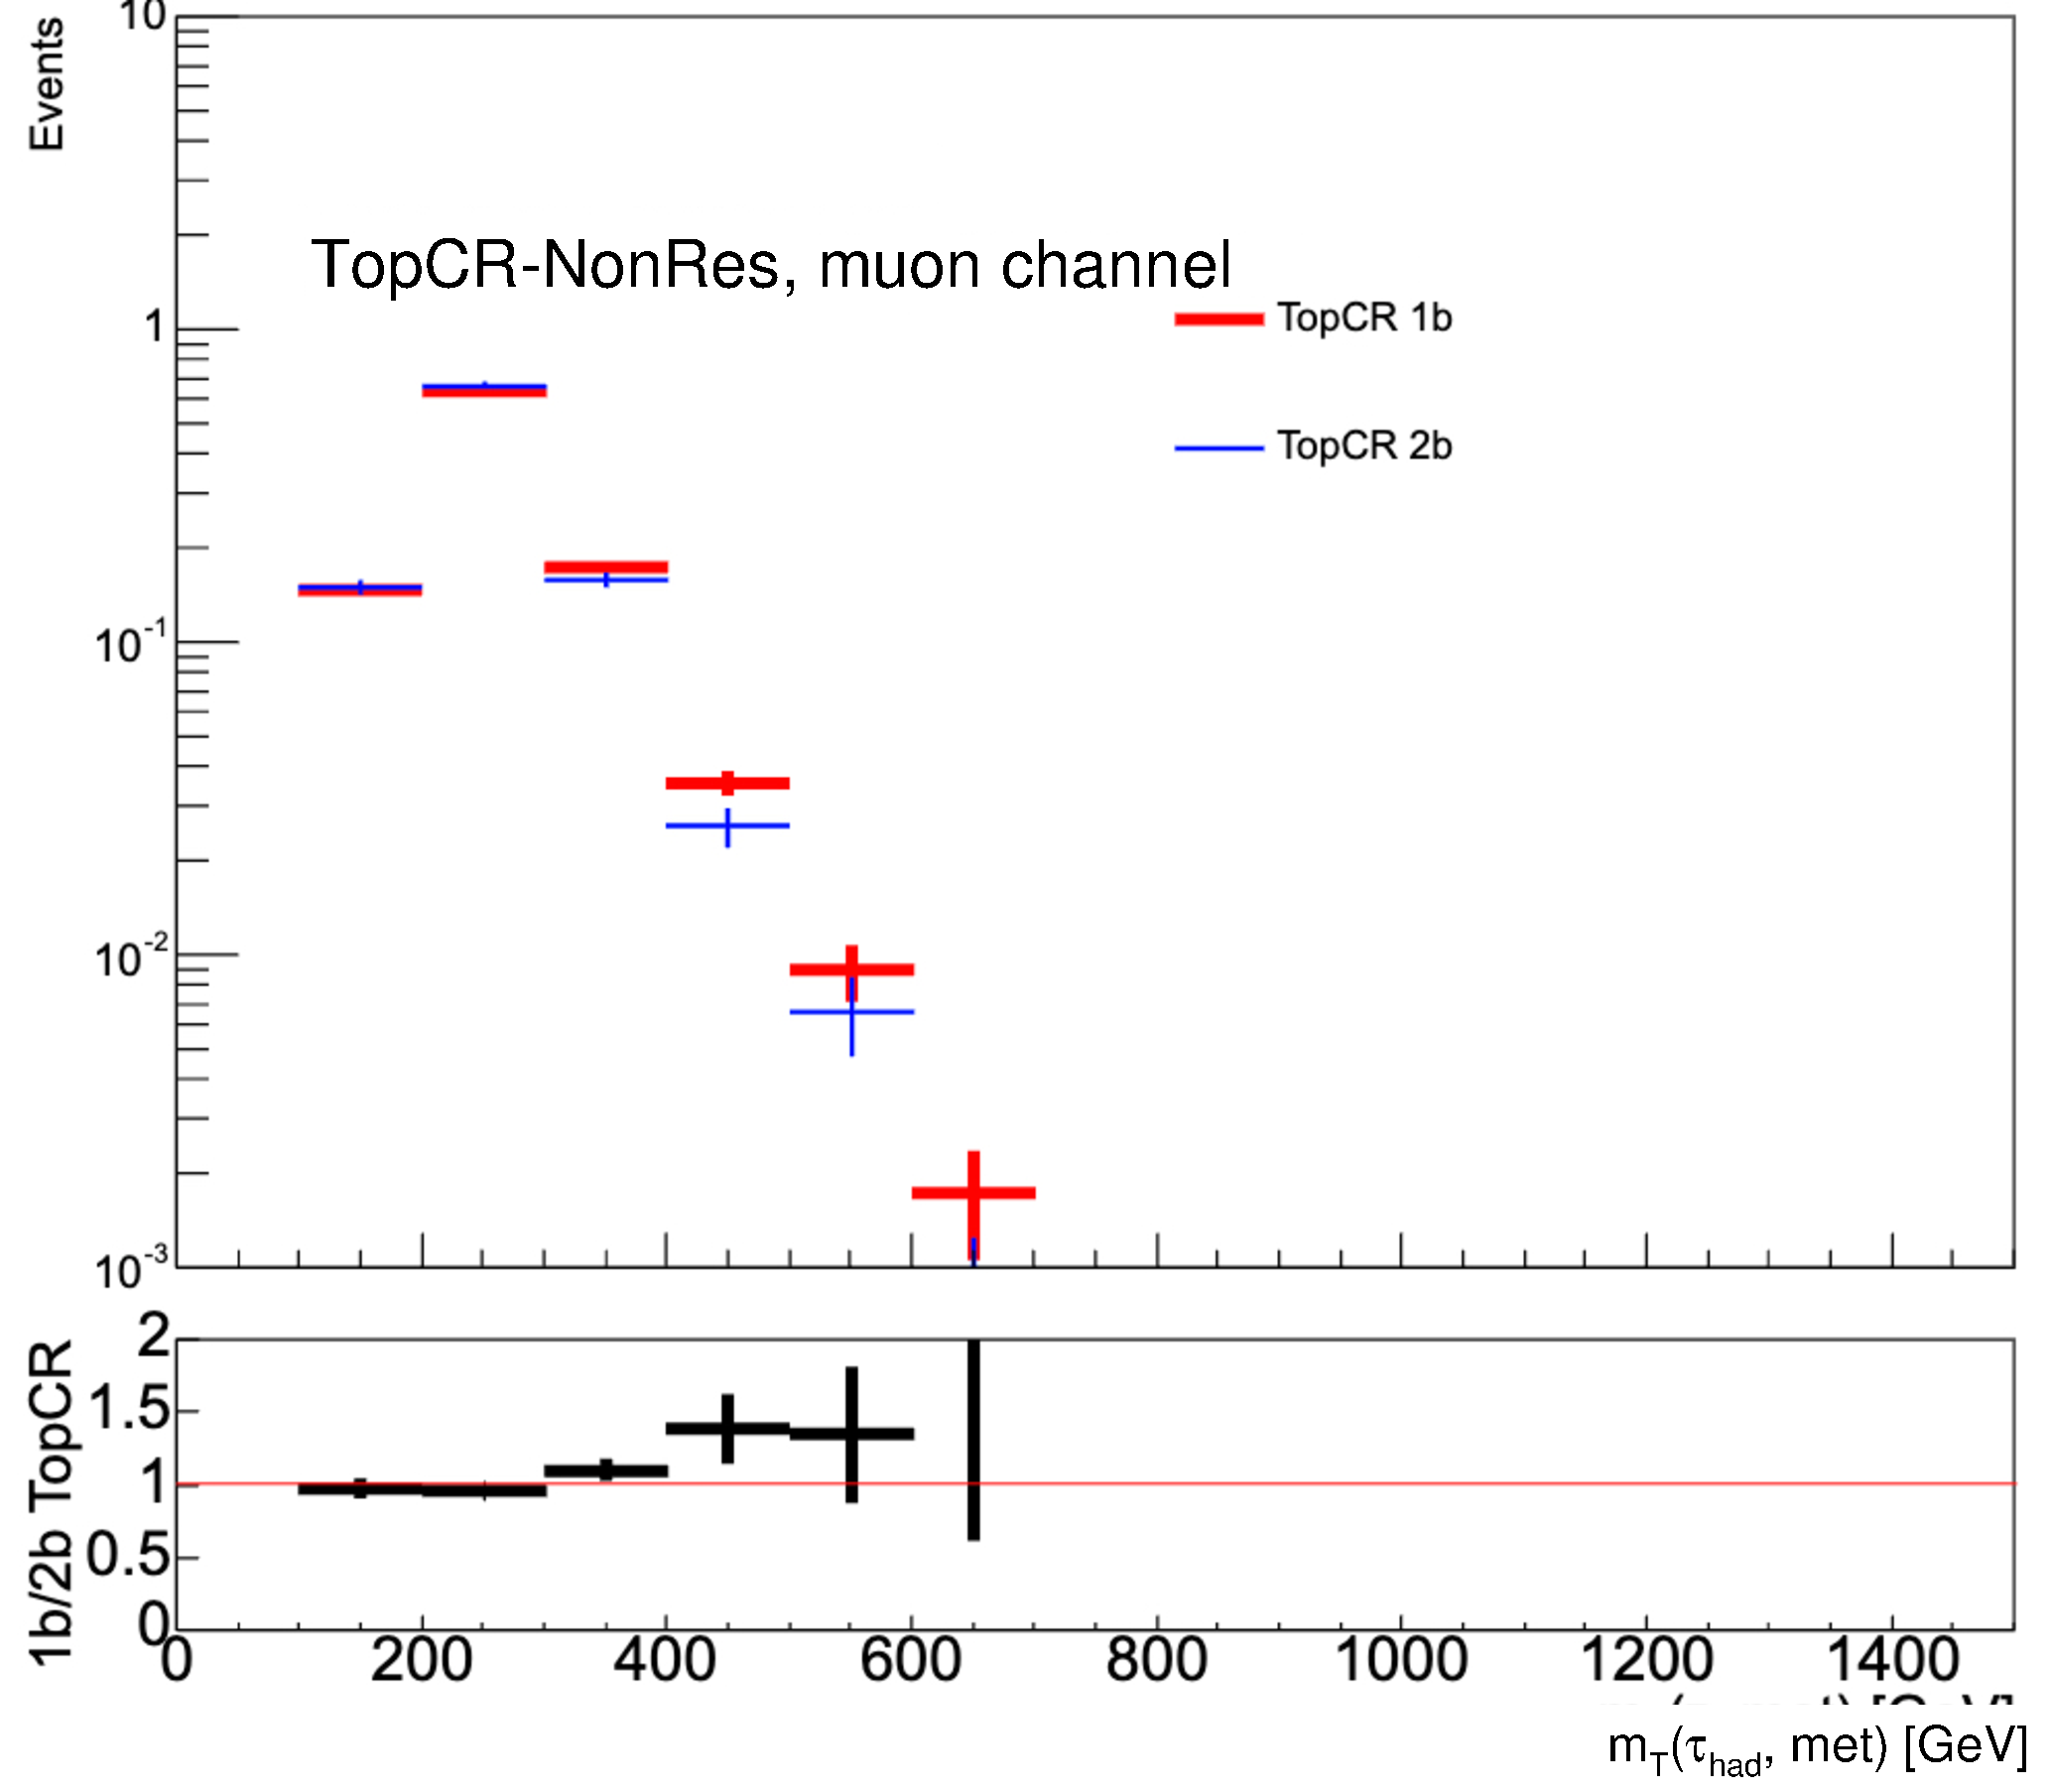
\includegraphics[width=\linewidth]{Figs/CH8/studies/TopCR_1mu_tch_mT.pdf}
        \caption[]{$\mu$ channel, NonRes.}
    \end{subfigure}
    \caption[One- and two-b-jet comparison of transverse mass]{Simulated $\mT$ distributions in the one- and two-$b$-jet $\CRTop$ samples. Each distribution is normalised to unit area. The red and blue lines represent the one- and two-$b$-jet samples, respectively. The electron and muon channels are shown for both topologies.}
    \label{fig:ch8_top_1b2b_mt}
\end{figure}

\begin{figure}[htpb]
    \centering
    \begin{subfigure}{0.49\linewidth}
        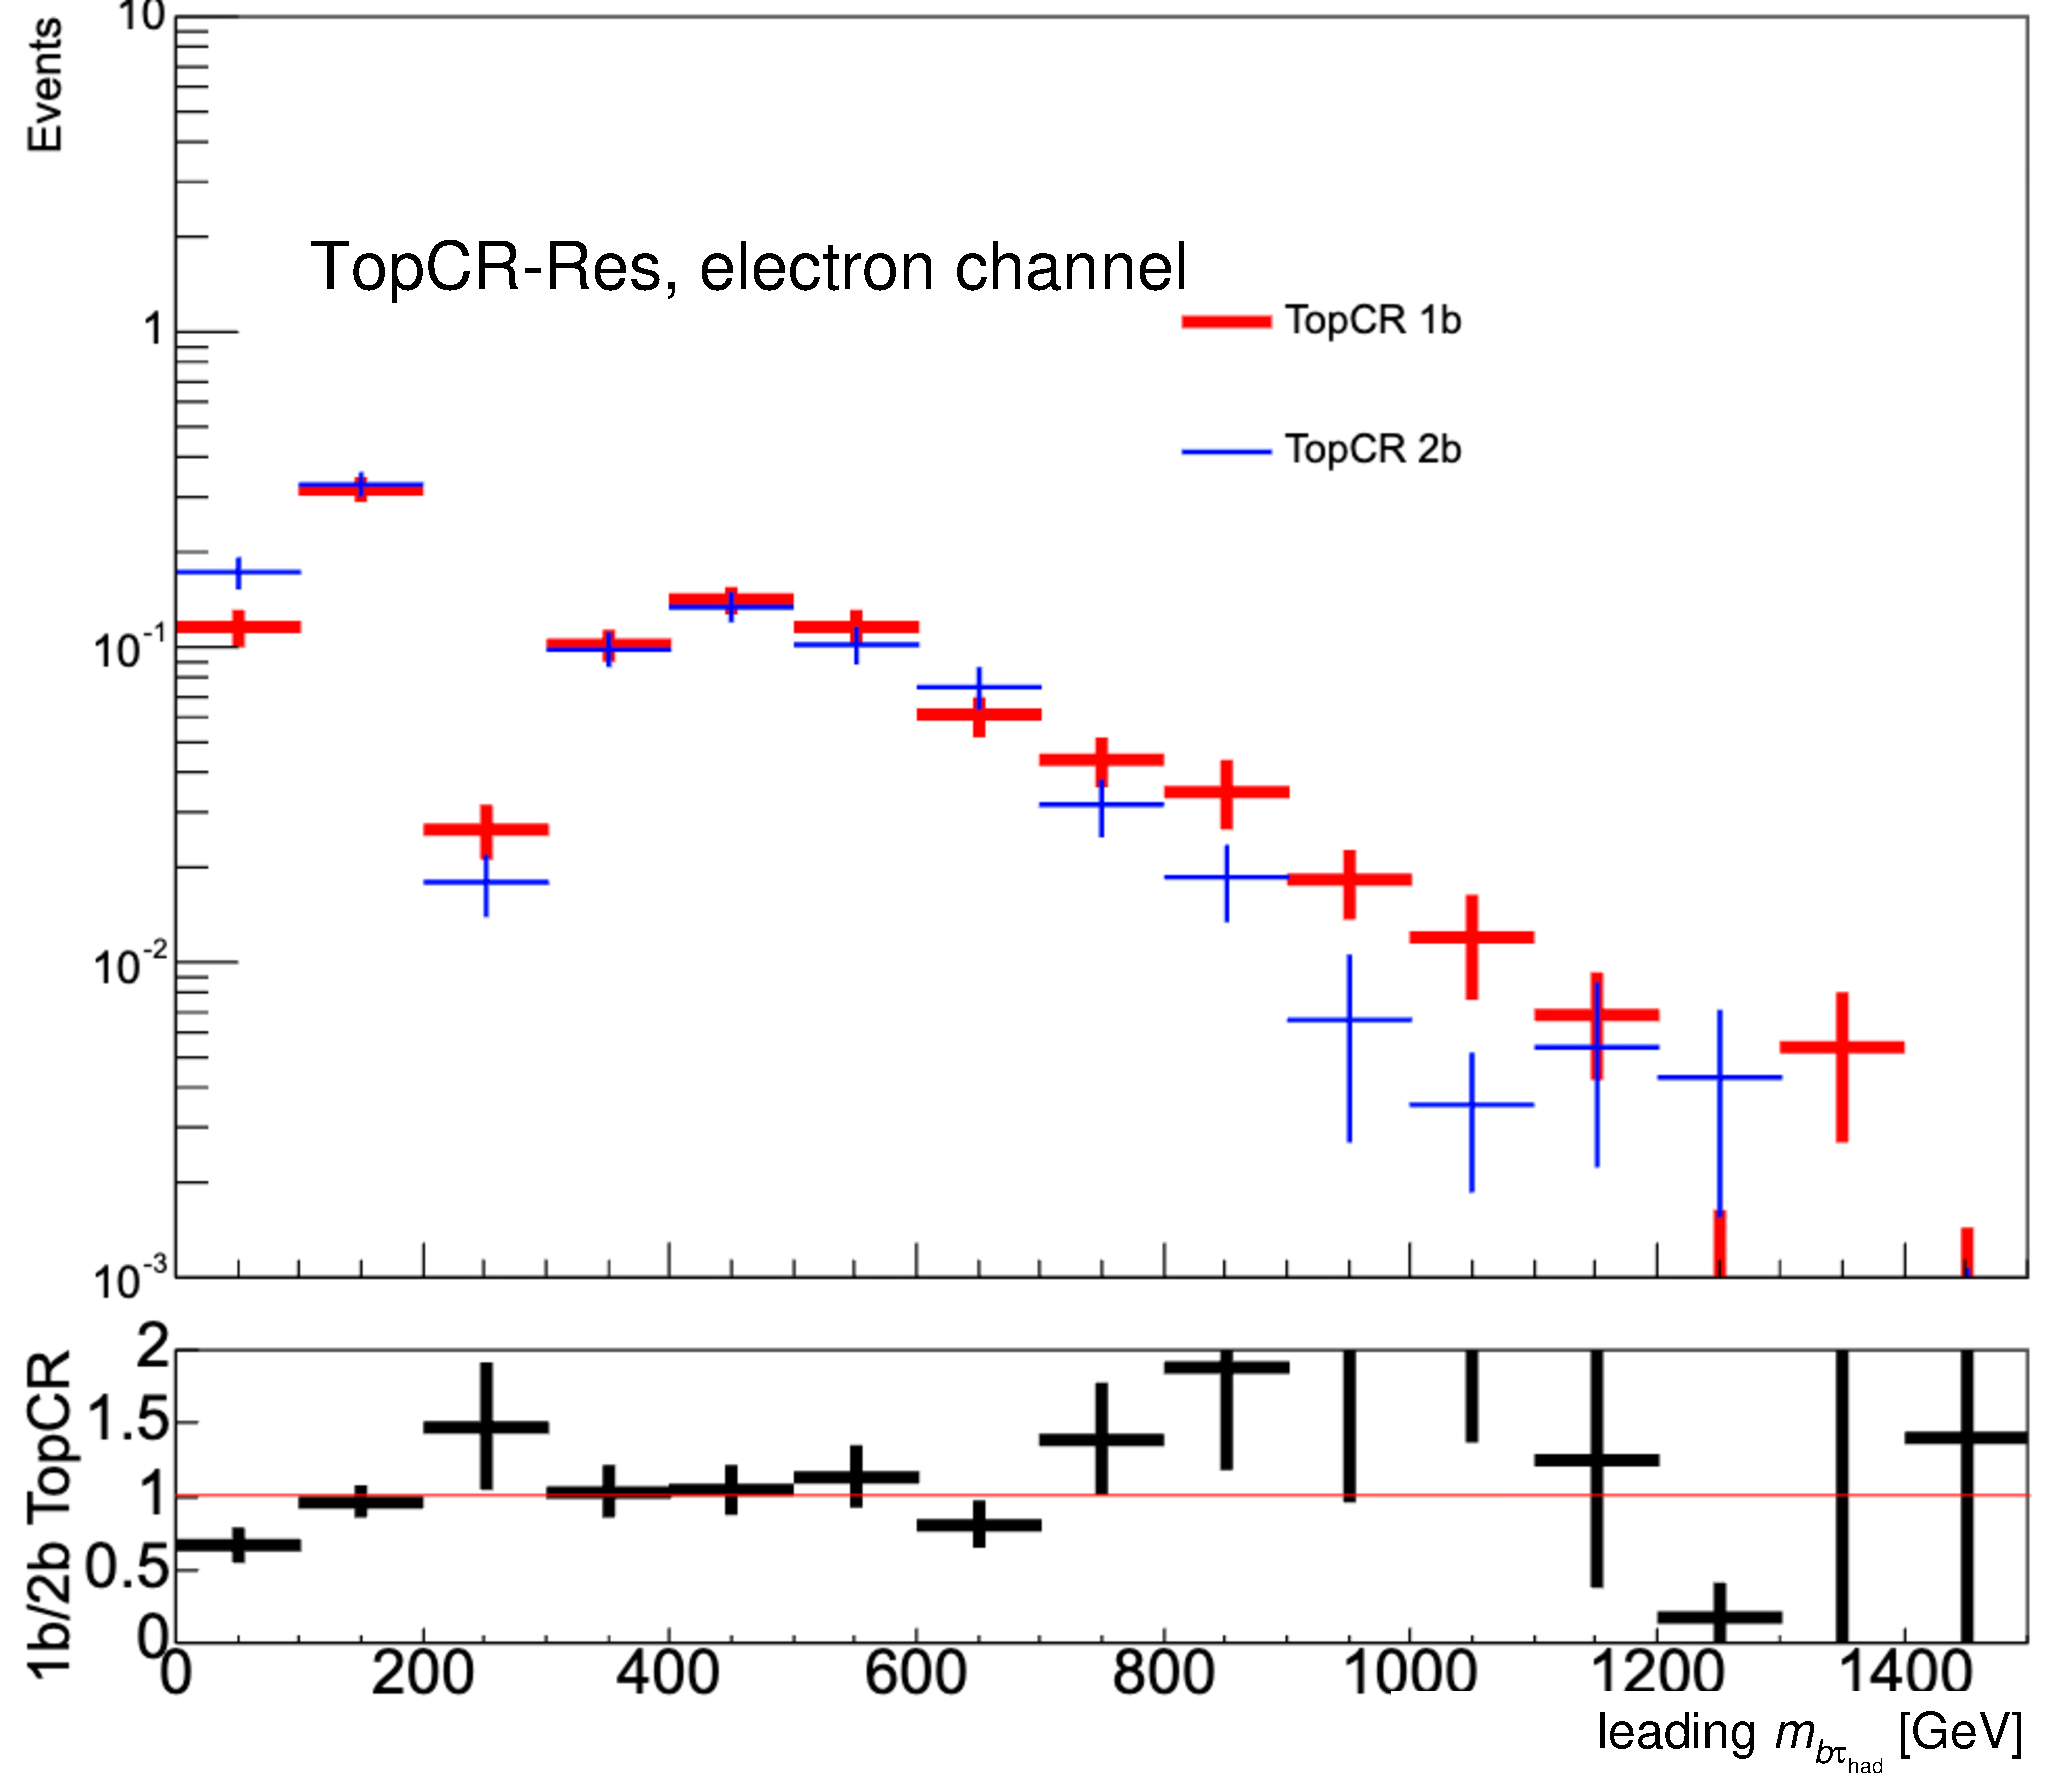
\includegraphics[width=\linewidth]{Figs/CH8/studies/TopCR_1e_sch_InvM.pdf}
        \caption[]{$e$ channel, Res.}
    \end{subfigure}\hfill
    \begin{subfigure}{0.49\linewidth}
        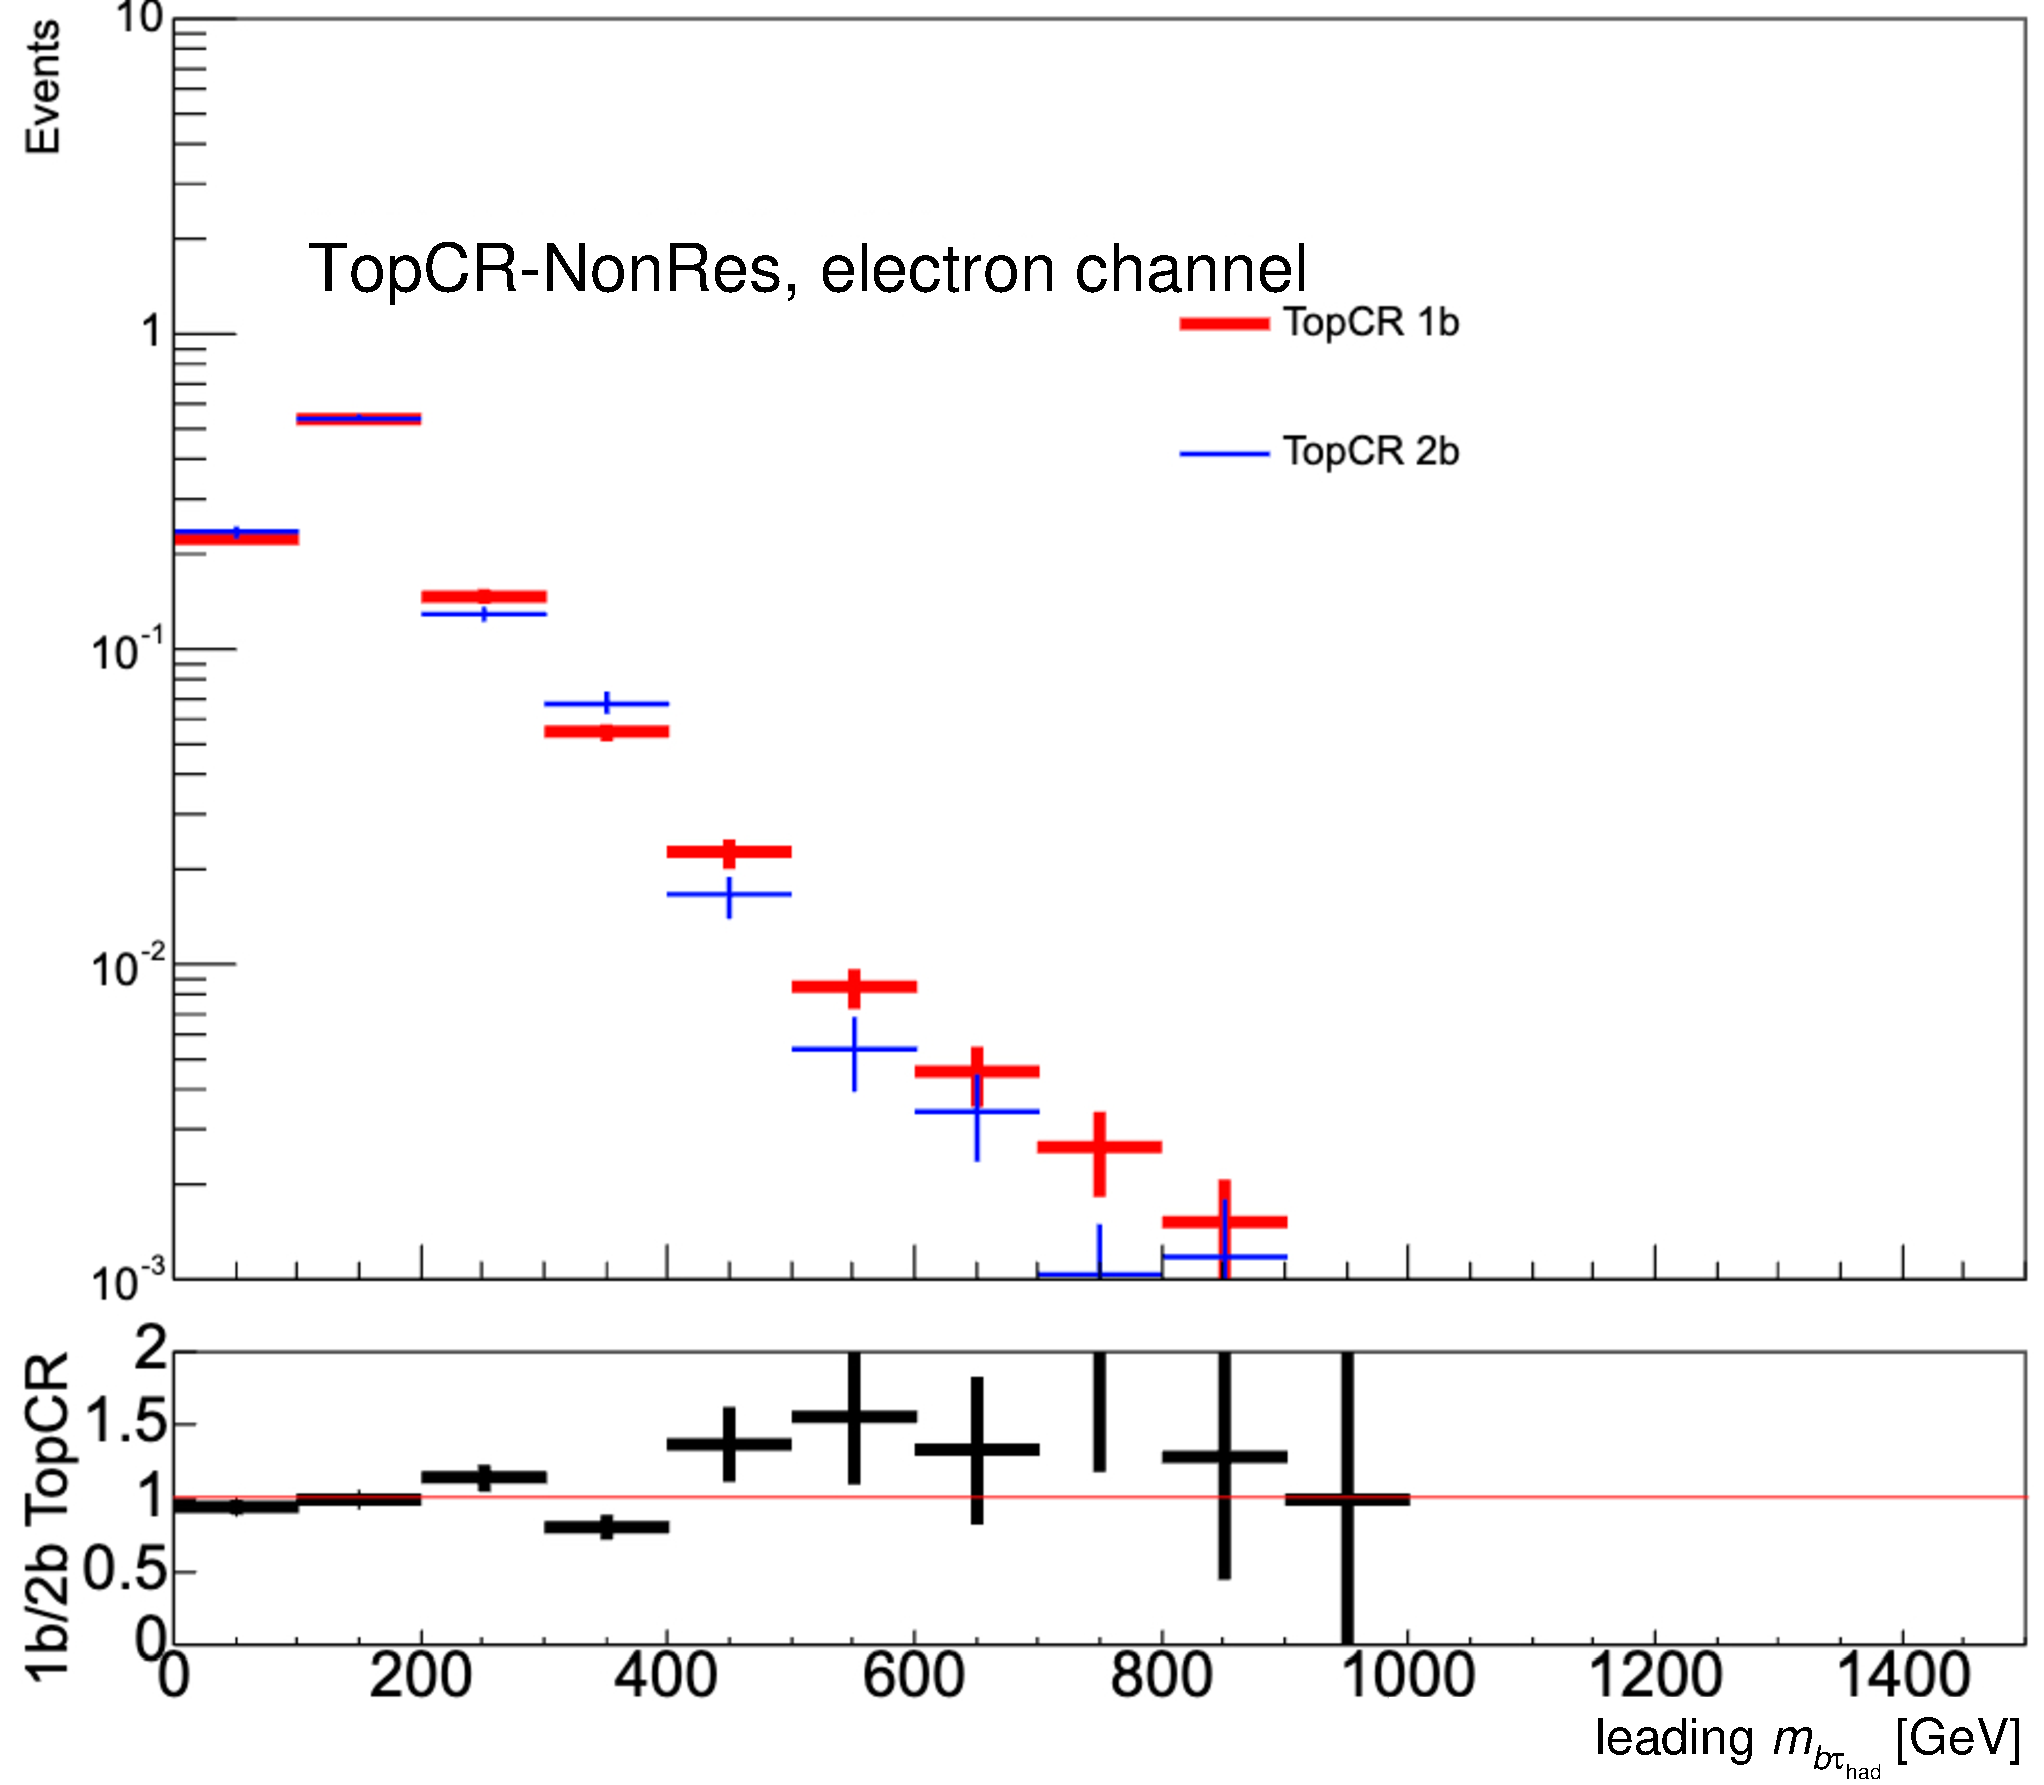
\includegraphics[width=\linewidth]{Figs/CH8/studies/TopCR_1e_tch_InvM.pdf}
        \caption[]{$e$ channel, NonRes.}
    \end{subfigure}\\
    \begin{subfigure}{0.49\linewidth}
        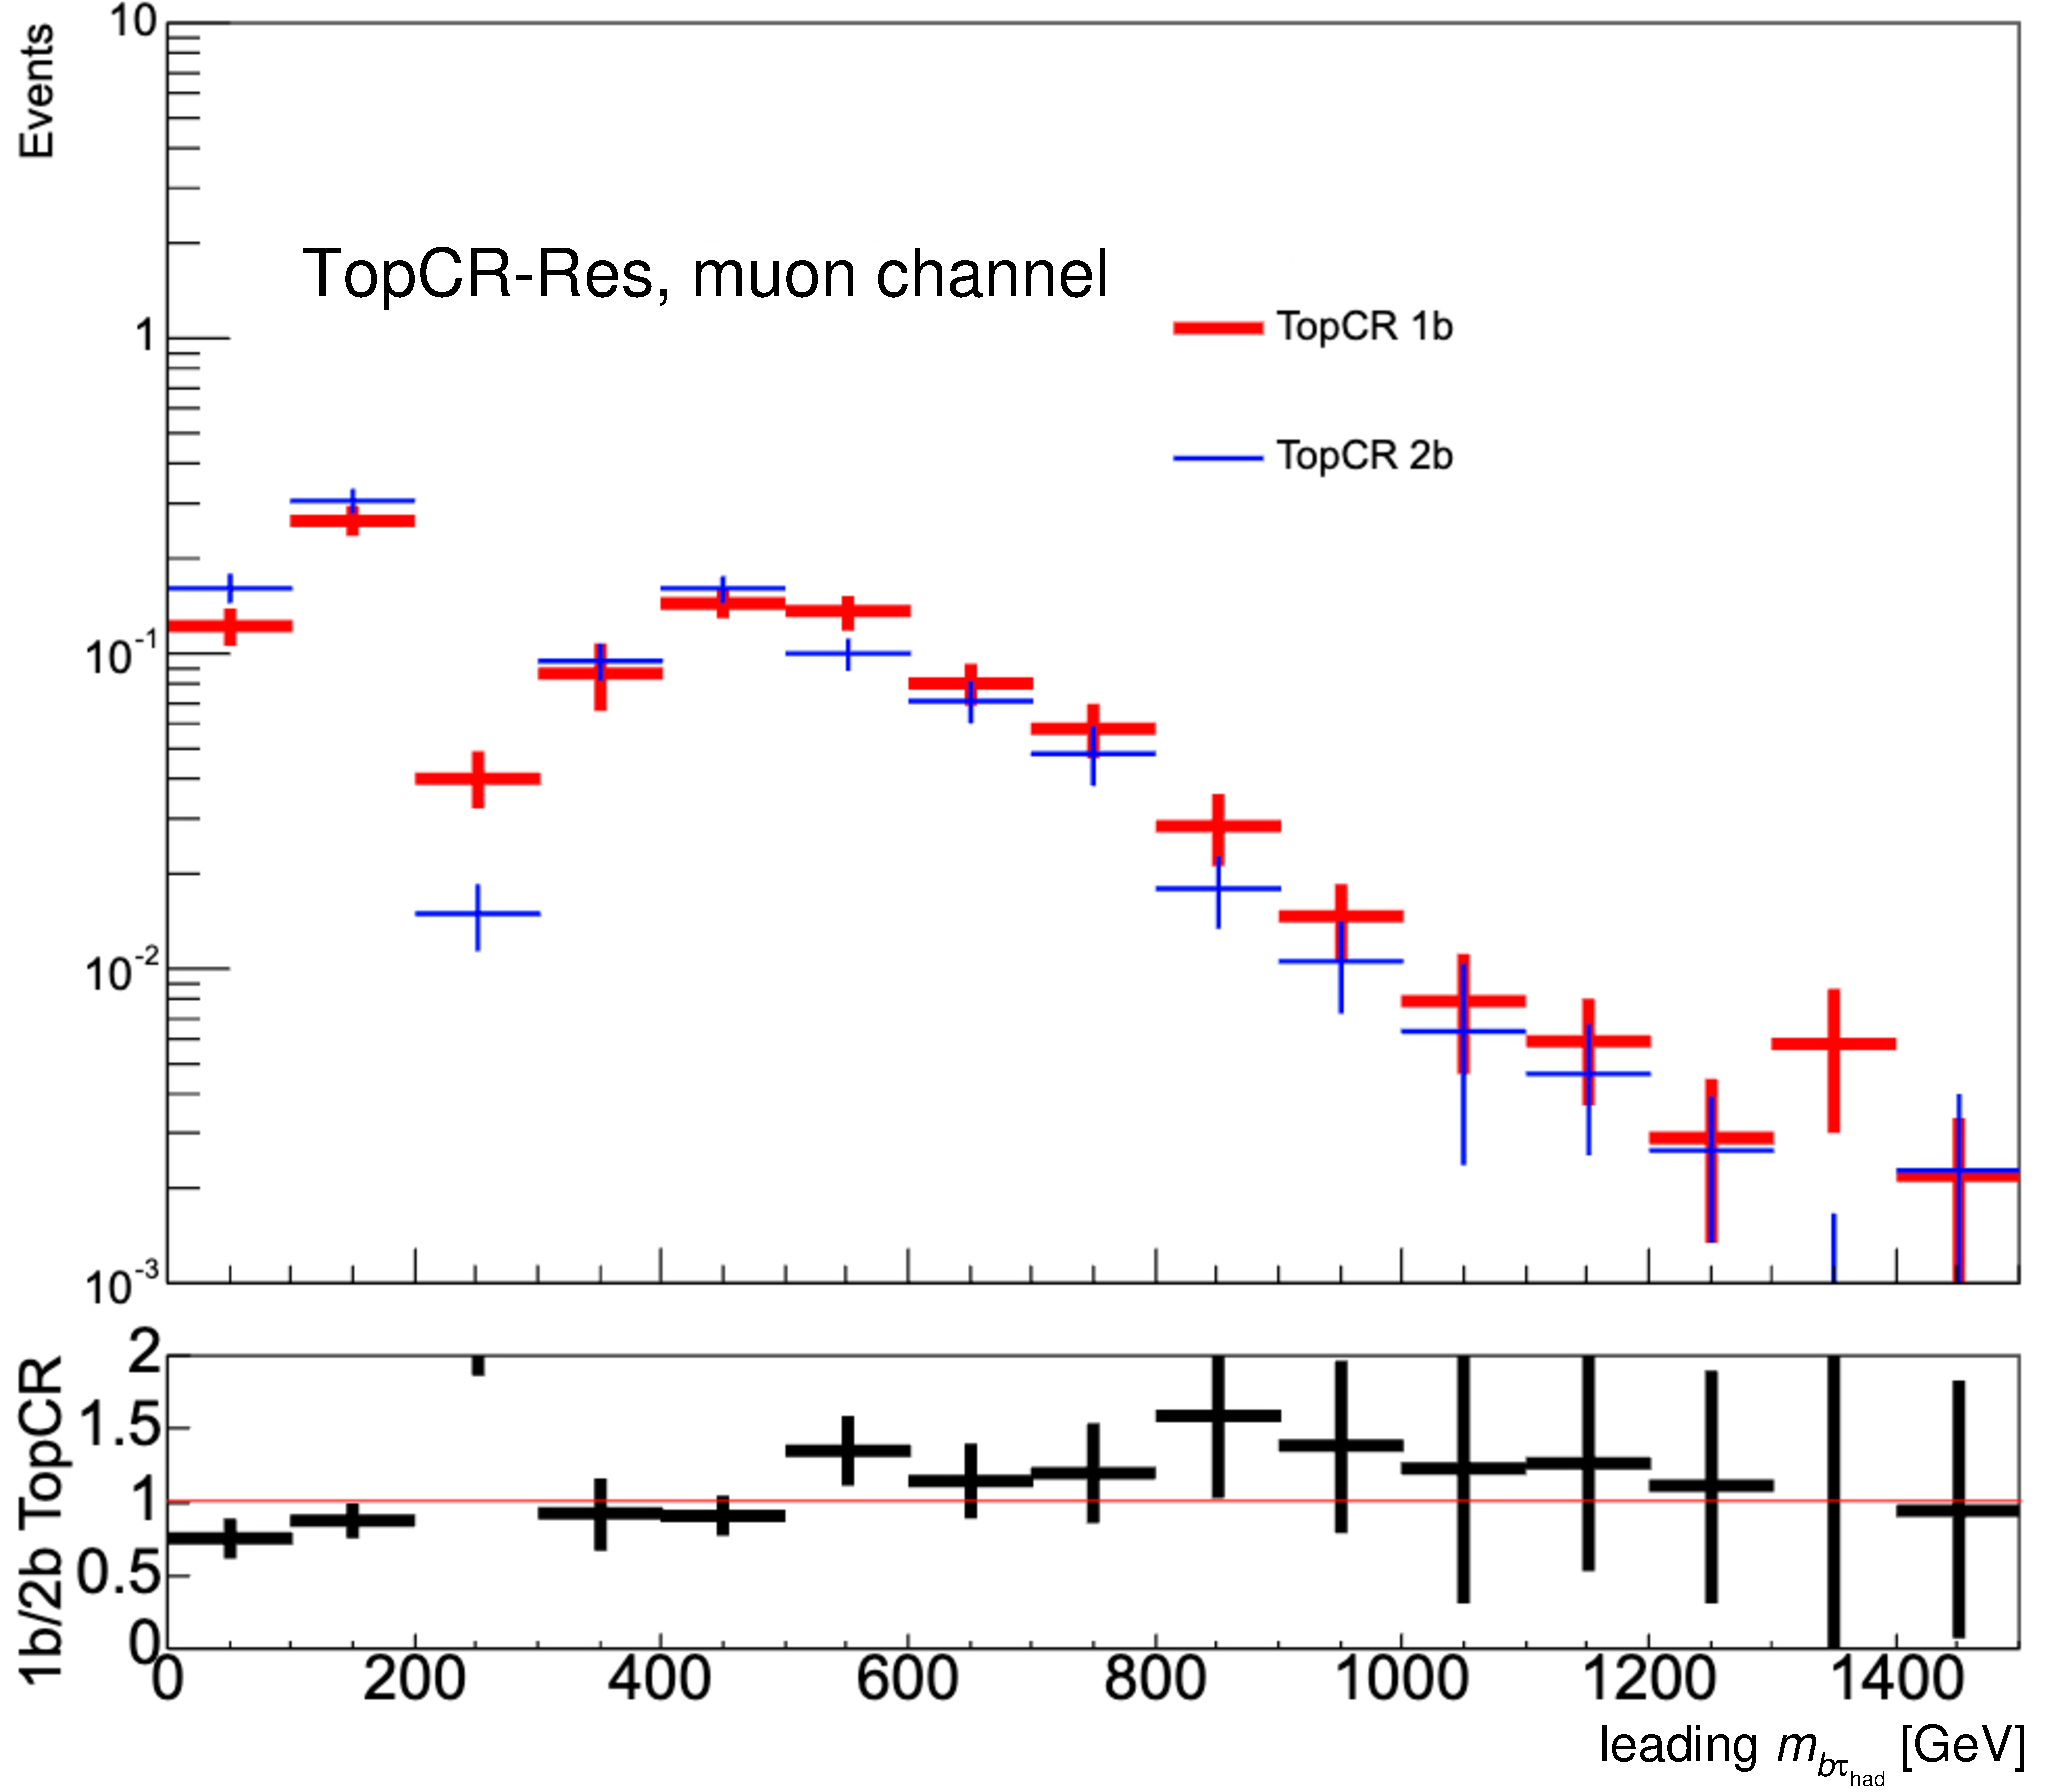
\includegraphics[width=\linewidth]{Figs/CH8/studies/TopCR_1mu_sch_InvM.pdf}
        \caption[]{$\mu$ channel, Res.}
    \end{subfigure}\hfill
    \begin{subfigure}{0.49\linewidth}
        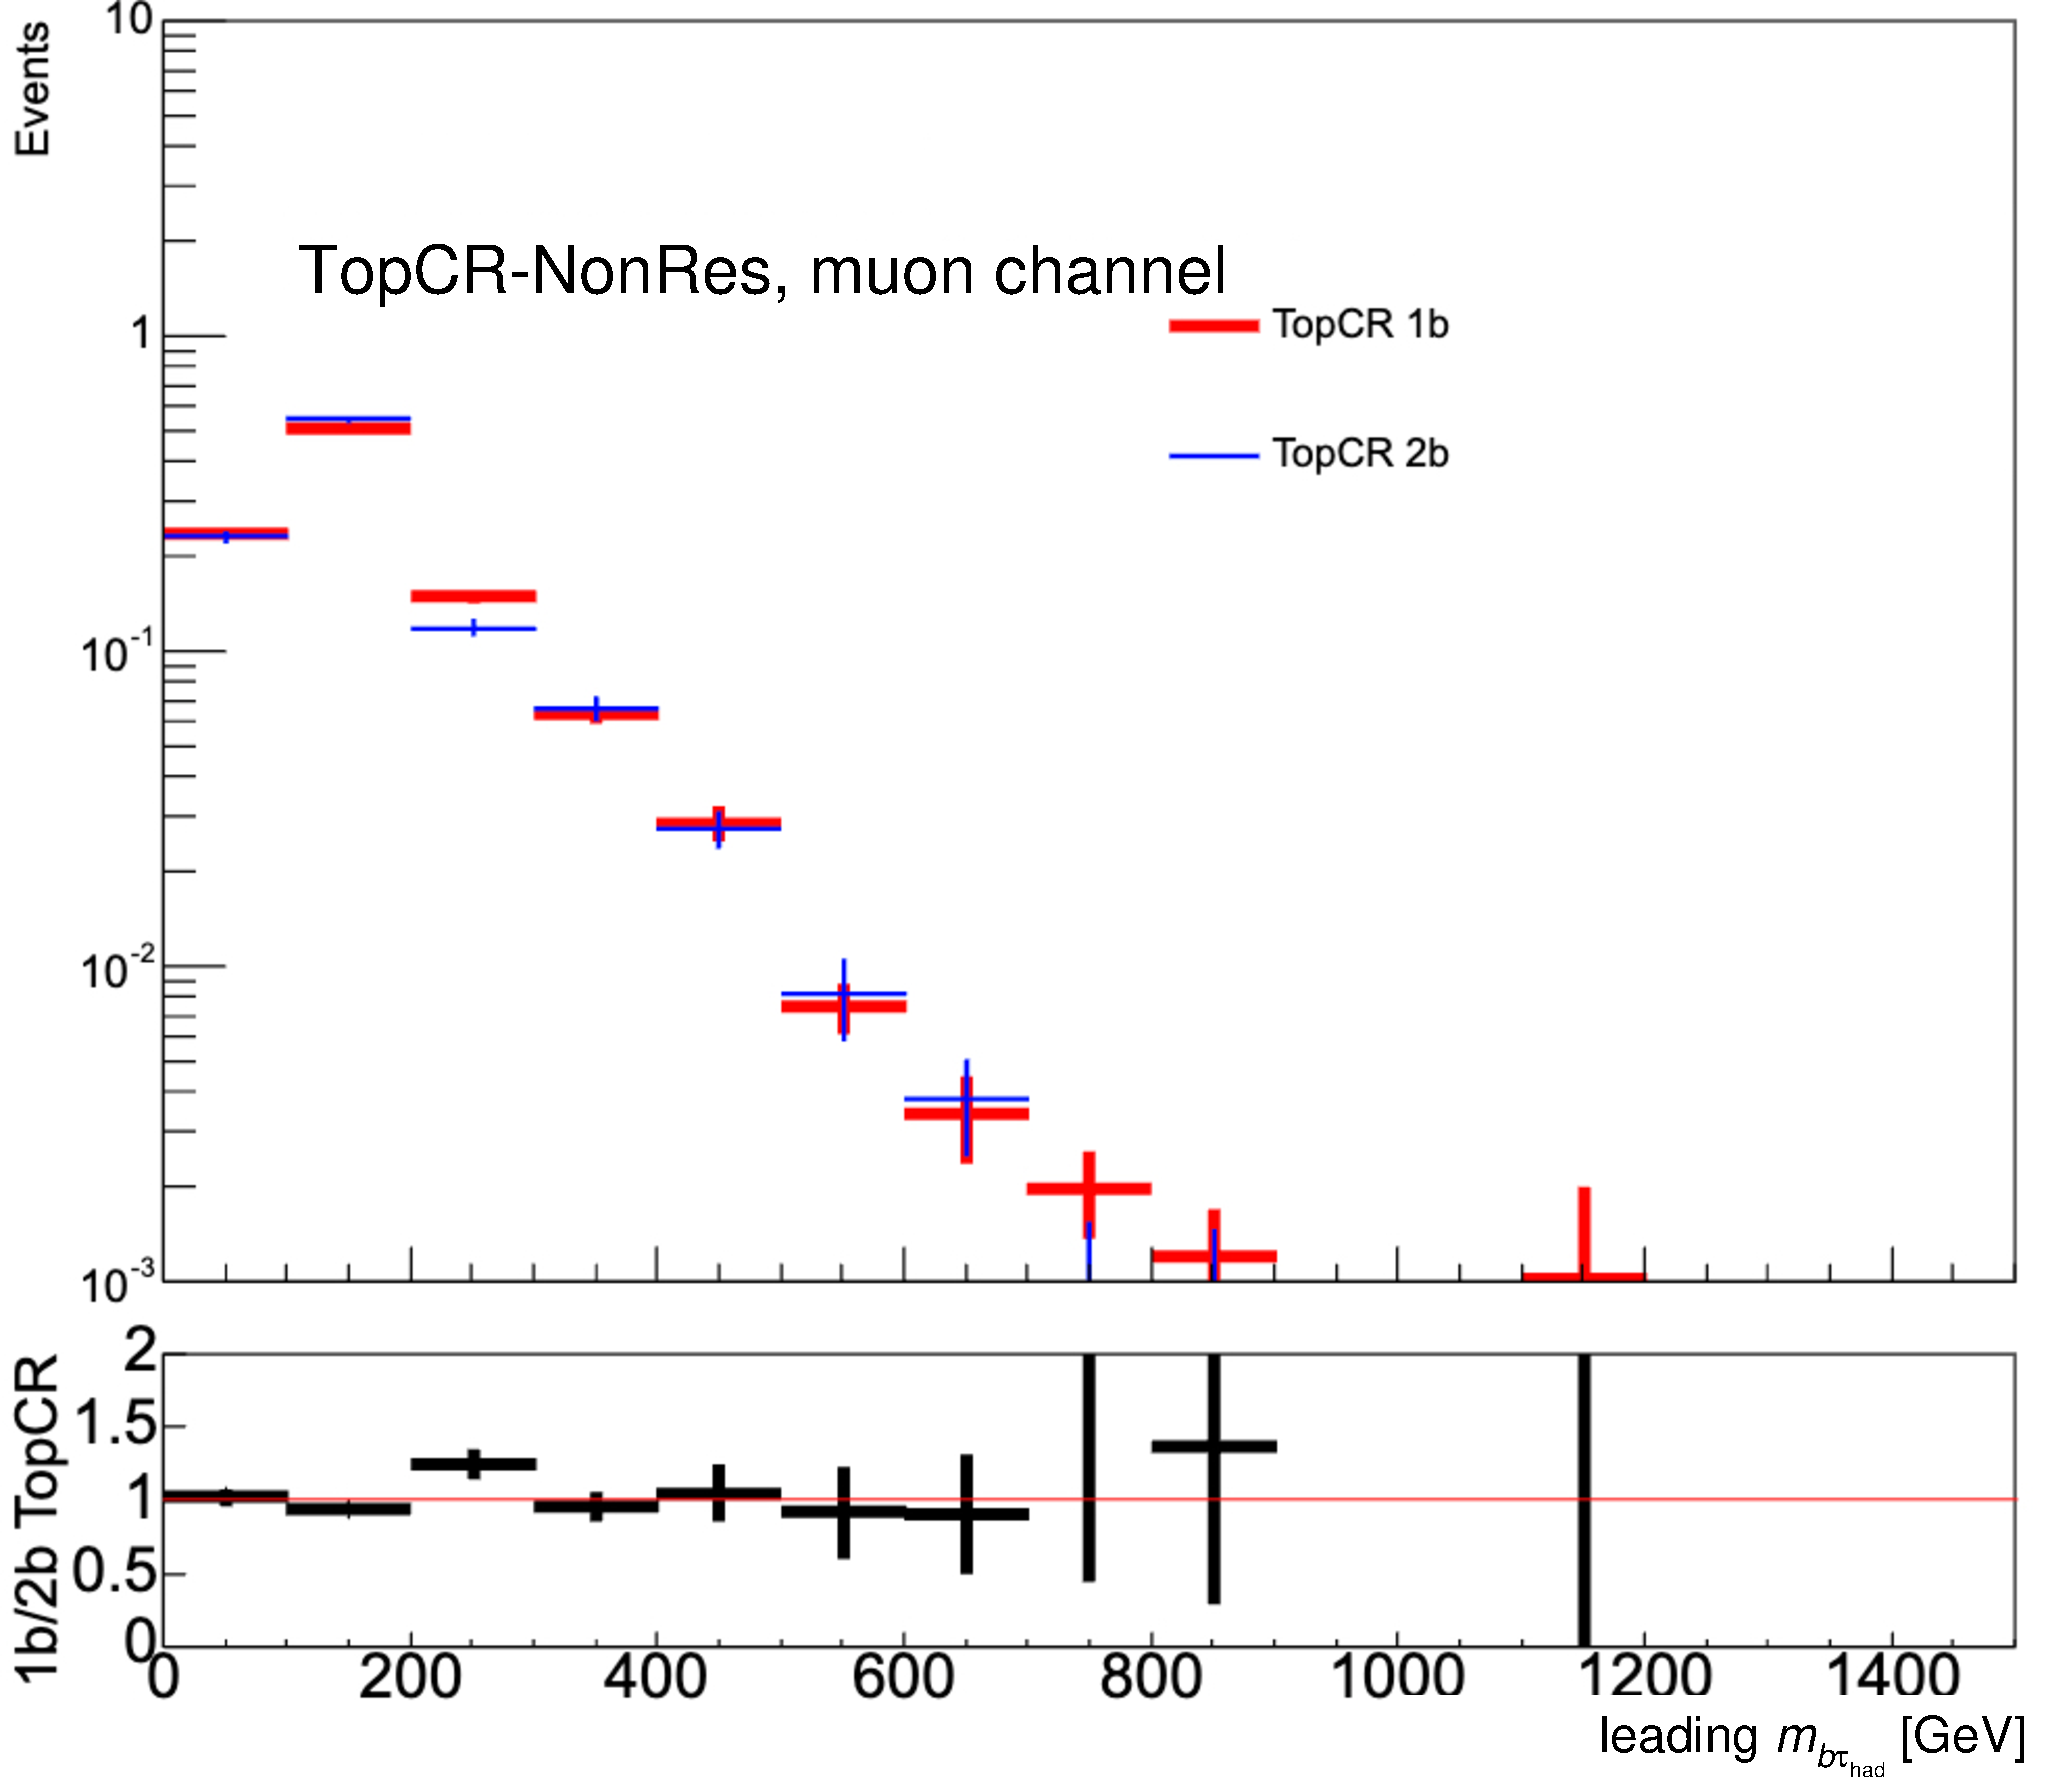
\includegraphics[width=\linewidth]{Figs/CH8/studies/TopCR_1mu_tch_InvM.pdf}
        \caption[]{$\mu$ channel, NonRes.}
    \end{subfigure}
    \caption[One- and two-b-jet comparison of tau-jet mass]{Simulated $m_{b\hadtau}$ distributions in the one- and two-$b$-jet $\CRTop$ samples. Each distribution is normalised to unit area. The red and blue lines represent the one- and two-$b$-jet samples, respectively. The electron and muon channels are shown for both topologies.}
    \label{fig:ch8_top_1b2b_mass}
\end{figure}


